\documentclass[dvipdfmx]{report} % 文章の形式を設定
\usepackage[margin=2.5cm]{geometry} % 書式の空白を設定
\usepackage[utf8]{inputenc} % 文字コードをUTF-8に設定
\usepackage{hyperref} % 目次にリンクを付けるため
\usepackage{lipsum} % ダミーテキスト用
\usepackage{tcolorbox} % 枠を利用するため
\usepackage{amsmath} % 数式の記述を行うため
\usepackage{bm} % ベクトルを太字で表示するため
\usepackage{graphicx} % 画像を表示するため
\usepackage{float} % 画像正しい位置で表示するため
\usepackage{tensor} % テンソルを記載するため
\usepackage{multicol} % 複数段落を作成するため
\usepackage{tikz} % 図を作成するため
\usepackage{enumerate} % リストを作成するため
\usepackage{amssymb} % 特殊文字を表示するため
\usepackage{color} % 文字の色を指定するため


\title{超大質量天体に落下する星の光学的出現}
\author{大豆生田 幹}
\date{}

\begin{document}

\maketitle % タイトルの作成
\tableofcontents % 目次の作成
\fontsize{11pt}{11pt}\selectfont % 文字サイズの指定

% =================================
% =================================
% =================================
% =================================
% =================================
% 一般相対論
% =================================
% =================================
% =================================
% =================================
% =================================
\chapter{一般相対論}


% =================================
% 概念
% =================================
\section{概念}
\textcolor{red}{いろいろ追記する。}

% =================================
% ベクトル
% =================================
\section{ベクトル}
時空は局所的に平坦とみなすことができた。つまり、時空は局所的にユークリッド空間と同相な空間と考えることができるので、その範囲では滑らかな座標が存在する。そこで、座標を以下のようにとることにする。
\[ (x^0, x^1, x^2, x^3) \]
時空上で実数値をもつ滑らかな関数$f(x^i)$と、実数$t$をパラメータとする曲線$C(t)$を考える。ここで、曲線$C(t)$上における関数$f(x^i)$の$t$微分は
\[ \frac{df}{dt} = \frac{\partial f}{\partial x^i} \frac{dx^i}{dt} \]
とかける。この右辺の成分それぞれに着目する。
座標変換$(x^0, x^1, x^2, x^3) \rightarrow (\bar{x}^0, \bar{x}^1, \bar{x}^2, \bar{x}^3)$を考えると
\begin{enumerate}[(1)\,]
\item{}
\[ v^i = \frac{dx^i}{dt} \]
では、
\begin{equation*}
\begin{split}
	\bar{v}^i &= \frac{d\bar{x}^i}{dt} = \sum_{j=0}^{3}\frac{\partial \bar{x}^i}{\partial x^j} v^j
\end{split}
\end{equation*}
このような関係を満たすものを反変ベクトルと言い、上記のようにベクトルの添え字を上に書く。
\item{}
\[ w_i = \frac{df}{dx^i} \]
では、
\begin{equation*}
\begin{split}
	\bar{w}_j = \frac{df}{d\bar{x}^i}  = \sum_{j=0}^{3}\frac{\partial x^i}{\partial \bar{x}^j} w_i
\end{split}
\end{equation*}
このような関係を満たすものを共変ベクトルと言い、上記のようにベクトルの添え字を下に書く。
\end{enumerate}
以上のことをアインシュタインの縮約規則(上付きの添え字と下付きの添え字は全て足し合わせることとする表現方法)を用いてまとめると、ベクトルは2種類に分類できて、それぞれの座標変換は以下のように書ける。
\begin{tcolorbox}[title=反変ベクトルの変換則]
	\[ \bar{v}^i = \frac{\partial \bar{x}^i}{\partial x^j} v^j \]
\end{tcolorbox}
\begin{tcolorbox}[title=共変ベクトルの変換則]
	\[ \bar{w}_i = \frac{\partial x_j}{\partial \bar{x}^i} w_j \]
\end{tcolorbox}
以降の数式は全て、アインシュタインの縮約規則を用いて表現している。

% =================================
% テンソル
% =================================
\section{テンソル}
ベクトルを定義したことで、そのベクトルが作る空間を考えることができる。
反変ベクトルの全体が作る空間を接ベクトル空間、共変ベクトルの全体が作る空間を双対接ベクトル空間と呼ぶ。それぞれの空間における基底を
\[ \bm{v}^j, \bm{w}_j \]
とおくと、そのテンソル積
\[ \bm{v}^i \otimes \bm{v}^j, \bm{v}^i \otimes \bm{v}^j \otimes \bm{w}_k \]
等で張られる線型空間を考えることができる。

\textcolor{red}{いろいろ追記する。(etc. テンソルの座標変換 反対称化)}


% =================================
% 計量
% =================================
\section{計量}
平面上のデカルト座標を$(x^1, x^2)$とおくと、そこでの線素(微小距離)は
\[ ds^2 = (dx^1)^2 + (dx^2)^2 \]
と書くことができる。これを$n$次元のデカルト座標$(x^1, x^2 \cdots x^{n-1}, x^n)$に拡張すると、線素は
\begin{equation*}
\begin{split}
	ds^2 = \delta_{ij} dx^i dx^j \\
	\left(
	\delta_{ij} =\
		\begin{cases}
			1 & (i=j)\\
			0 & (i \neq j)
		\end{cases}
	\right)
\end{split}
\end{equation*}
と書くことができる。さらに一般の曲がった次元に拡張すると、線素は
\[ ds^2 = g_{ij} dx^i dx^j \]
と書くことができる。この$g_{ij}$を「計量」と呼び、これがまさに時空を定義する量である。座標変換$(x^0, x^1, x^2, x^3) \rightarrow (\bar{x}^0, \bar{x}^1, \bar{x}^2, \bar{x}^3)$を考えると、線素は座標変換に対して不変なので
\begin{equation*}
\begin{split}
	ds^2 &= g_{ij} dx^i dx^j \\
	&= \bar{g}_{kl} d \bar{x}^k d \bar{x}^l\\
	&= \bar{g}_{kl} \left( \frac{\partial \bar{x}^k}{\partial x^i} dx^i \right) \left( \frac{\partial \bar{x}^l}{\partial x^j} dx^j \right)
\end{split}
\end{equation*}
よって、以下のことがわかる。
\begin{tcolorbox}[title=計量$g_{ij}$の変換則]
	\[ \bar{g}_{kl} \frac{\partial \bar{x}^k}{\partial x^i} \frac{\partial \bar{x}^l}{\partial x^j} = g_{ij} \]
\end{tcolorbox}
変換則より、計量$g_{ij}$は2階の共変テンソルとわかる。$g_{ij}$の逆行列$g^{ij} = (g^{-1})_{ij}$を考えると
\begin{equation*}
\begin{split}
	\left( \bar{g}_{kl} \frac{\partial \bar{x}^k}{\partial x^i} \frac{\partial \bar{x}^l}{\partial x^j} \right) g^{ij} &= g_{ij} g^{ij}\\
	\left( \bar{g}_{kl} \frac{\partial \bar{x}^k}{\partial x^i} \frac{\partial \bar{x}^l}{\partial x^j} \right) g^{ij} &= I\\
\end{split}
\end{equation*}
この整合性$I = I$を考えると
\begin{tcolorbox}[title=計量$g^{ij}$の変換則]
	\[ \bar{g}^{kl} \frac{\partial x^i}{\partial \bar{x}^k} \frac{\partial x^j}{\partial \bar{x}^l} = g^{ij} \]
\end{tcolorbox}
変換則より、計量$g^{ij}$は2階の反変テンソルとわかる。

\textcolor{red}{添え字の上げ下げについて記載する}


% =================================
% 内積
% =================================
\section{内積}
任意の2つのベクトル$\vec{A}, \vec{B}$それぞれの成分$A^i, B^i$とおいて、一般の曲がった次元での内積は
\[ \vec{A} \cdot \vec{B} = g_{ij} A^i B^j \]
と定義する。


% =================================
% 並行移動
% =================================
\section{並行移動}
曲がった時空上でベクトルの並行移動を考える。ある点$x$のベクトル$A^i(x)$を微小変位$\delta x$だけ離れた$x + \delta x $に並行移動したベクトル$A^i_{/\!/}(x + \delta x)$を以下のように書くことにする。
\[ A^i_{/\!/}(x + \delta x) = A^i(x) - \tensor{\Gamma}{^i_{jk}}(x) A^j(x) \delta x^k \]
ここで導入した$\tensor{\Gamma}{^i_{jk}}(x)$を接続とよび、この量を適切に定義することでベクトルの並行移動を定義する。
\begin{figure}[H]
    \centering
    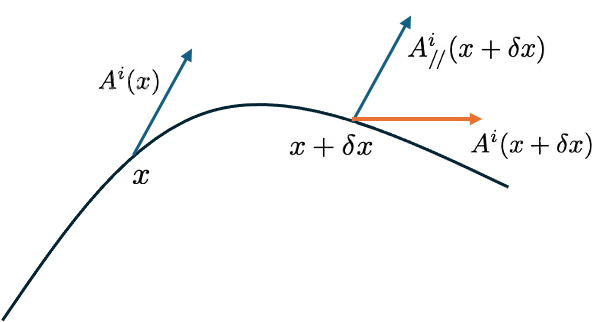
\includegraphics[width=0.5\columnwidth]{./images/0106/01.png}
    \caption{並行移動}
    \label{}
\end{figure}
並行移動が満たすべき条件は2つ考えられる。
\begin{enumerate}[(1)\,]
\item{並行移動によって任意の2つのベクトルの内積が保たれる}\\
この条件により
\begin{equation*}
\begin{split}
	g_{ij}(x) A^i (x) B^j (x) &= g_{ij}(x + \delta x) A^i_{/\!/} (x + \delta x) B^j_{/\!/} (x + \delta x)\\
	&= \left
	
\end{split}
\end{equation*}
\item{並行移動によって任意の2つのベクトルにねじれが生じない}
\end{enumerate}


\[ \tensor{\Gamma}{^i_{[jk]}} = 0 \]

% =================================
% 共変微分
% =================================
\section{共変微分}


% =================================
% 曲率
% =================================
\section{曲率}


% =================================
% 測地線
% =================================
\section{測地線}


% =================================
% アインシュタイン方程式
% =================================
\section{アインシュタイン方程式}


% =================================
% シュバルツシルトの外部解
% =================================
\section{シュバルツシルトの外部解}


% =================================
% =================================
% =================================
% =================================
% =================================
% シュバルツシルト時空における軌道
% =================================
% =================================
% =================================
% =================================
% =================================
\chapter{シュバルツシルト時空における天体の軌道}
\section{軌道の安定性}


/////////////////////////////////////////////////////////////////////////\\
/////////////////////////////////////////////////////////////////////////

% 方程式
\begin{equation*}
\begin{split}
	\bar{w}_j = \left( \right) \int^{}_{}
\end{split}
\end{equation*}

% ボックス
\begin{tcolorbox}[title=メモ用]
\begin{eqnarray*}
	1 = 0
\end{eqnarray*}
\end{tcolorbox}

% { 付き方程式
\begin{equation}
\left\{ \,
\begin{aligned}
	1 &= 0\\
	1 &= 0\\
\end{aligned}
\right.
\end{equation}

% 画像
\begin{figure}[H]
    \centering
    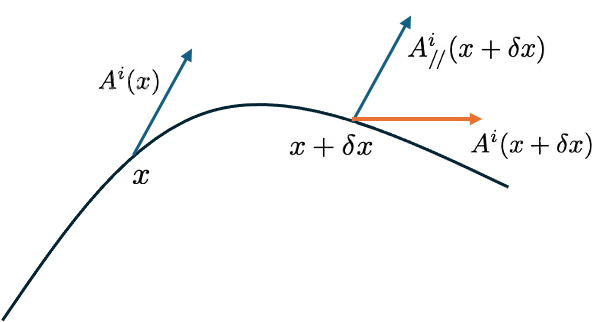
\includegraphics[width=0.5\columnwidth]{./images/0106/01.png}
    \caption{並行移動}
    \label{}
\end{figure}

% リスト
\begin{enumerate}[(1)\,]
\item{}
\end{enumerate}

\end{document}